\documentclass[t]{beamer}
\usepackage{beamerthemesplit}
\usepackage{pstricks}
\usepackage{graphicx}
\usepackage{hyperref}
\usepackage{subfigure}
\usepackage{multirow}
\usepackage{xspace}
\usepackage{listings}


\mode<presentation>
{ \usetheme{Boadilla}
  \setbeamercovered{transparent}
  \setbeamertemplate{items}[circle]
  \setbeamertemplate{theorems}[numbered]
  \setbeamertemplate{footline}[frame number]
}
 
%\useinnertheme[shadow=true]{rounded}
\useoutertheme{shadow}
\usecolortheme{whale}

\def\answer{ANS}


\newcommand\blfootnote[1]{
  \begingroup
  \renewcommand\thefootnote{}\footnote{#1}
  \addtocounter{footnote}{-1}
  \endgroup
}

\mode
<all>

\title{C Programming: lab}
\author{Wan-Lei Zhao}

\makeatletter

\begin{document}
\begin{frame}
   \begin{center}
    \vspace{24pt}
    \Huge\textbf{C Programming}\blfootnote{Email: wlzhao@xmu.edu.cn, copyrights are fully preserved by the author.}\\
     \Huge{\mbox{Lab 6: Functions and Array}}
    \vspace{36pt}
  \end{center}
  \begin{align*}
   \vspace{18pt}
      \large{\mbox{Lecturer:}~Dr.~\mbox{Wan-Lei~~Zhao}} \\
      \large{Spring~~Semester~~2022} \\
   \vspace{30pt}
  \end{align*}
\end{frame}

\definecolor{cornblue}{HTML}{6495ED}
\definecolor{navyblue}{HTML}{000080}
\definecolor{midnblue}{HTML}{191970}
\definecolor{lghtblue}{HTML}{B0C4DE}
\setbeamercolor{background}{fg=black, bg=lghtblue}
\setbeamercolor{palette primary}{fg=white, bg=lghtblue}
\setbeamercolor{palette secondary}{fg=black, bg=cornblue}
\setbeamercolor{palette tertiary}{fg=black, bg=lghtblue}
\setbeamercolor{palette quaternary}{fg=black, bg=lghtblue}
\setbeamercolor{frametitle}{fg=black, bg=white}
\definecolor{ballblue}{rgb}{0.13, 0.67, 0.8}
\definecolor{cornflowerblue}{rgb}{0.39,0.58,0.93}
\definecolor{babyblueeyes}{rgb}{0.63, 0.79, 0.95}

\setbeamertemplate{footline}
{
  \leavevmode%
  \hbox{%
  \begin{beamercolorbox}[wd=.275\paperwidth,ht=2.25ex,dp=1ex,center]{author in head/foot}%
    \usebeamerfont{author in head/foot}\insertshortauthor
  \end{beamercolorbox}%
  \begin{beamercolorbox}[wd=.44\paperwidth,ht=2.25ex,dp=1ex,center]{title in head/foot}%
    \usebeamerfont{title in head/foot}\insertshorttitle\hspace*{3em}
    \hspace*{1ex}
  \end{beamercolorbox}%
  \begin{beamercolorbox}[wd=.285\paperwidth,ht=2.25ex,dp=1ex,center]{date/foot}%
    \usebeamerfont{title in head/foot}\hspace*{2em}
    \insertframenumber{} / \inserttotalframenumber\hspace*{1ex}
  \end{beamercolorbox}}%
  \vskip0pt
}



% preset-listing options
\lstset{
  backgroundcolor=\color{white},   
  basicstyle=\footnotesize,    
  language=c,
  breakatwhitespace=false,         
  breaklines=true,                 % sets automatic line breaking
  captionpos=b,                    % sets the caption-position to bottom
  commentstyle=\color{ballblue},    % comment style
  extendedchars=true,              
  frame=single,                    % adds a frame around the code     
  keywordstyle=\color{blue},       % keyword style
  numbers=left,                    
  numbersep=5pt,                   
  numberstyle=\tiny\color{blue}, 
  rulecolor=\color{babyblueeyes},
  stepnumber=1,              
  stringstyle=\color{black},     % string literal style
  tabsize=4,                       % sets default tabsize to 4 spaces
  title=\lstname                   
}


\section{Functions}
\label{sec:func}
\begin{frame}<beamer>
    \frametitle{Outline}
    \tableofcontents[currentsection]
\end{frame}

\begin{frame}{Narcissus number}
\begin{itemize}
	\item {Work out Narcissus number of 3 digits (100 $\sim$ 999)}
	\item {3 digits number satisfies: $153=1^3+5^3+3^3$}
	\begin{enumerate}
		\item {function should be defined as `\textcolor{blue}{int} isNarcNum(\textcolor{blue}{int} a)'}
		\item {Call it in main function to check numbers from 100 to 999}
		\item {Print out all Narcissus number in this range}
		\item {Two numbers in each line}
	\end{enumerate}
\end{itemize}
\end{frame}

\ifx\answer\defined
\begin{frame}[fragile]{Narcissus number: the answer}
\begin{columns}
\begin{column}{0.5\linewidth}
\begin{lstlisting}[linewidth=0.95\linewidth, xleftmargin=0.05\linewidth]
#include <stdio.h>
int isNaciNum(int a)
{
   int h = 0, t = 0, d = 0;
   int s  = 0;
   h = a/100;
   t = (a%100)/10;
   d = a%10;
   s = h*h*h+t*t*t+d*d*d;
   if(s == a)
     return 1;
   else 
     return 0;
}
\end{lstlisting}
\end{column}
\begin{column}{0.5\linewidth}
\begin{lstlisting}[firstnumber=15]
int main()
{
   int i = 0, t = 0;
   for(i = 100; i <= 999; i++)
   {
       if(isNarcNum(i))
       {
           t++;
           printf("%3d ", i);
           if(t%3 == 0)
           {
              printf("\n");
           }
       }//if
   }//for()
}
\end{lstlisting}
\end{column}
\end{columns}
\end{frame}
\fi

\begin{frame}
\frametitle{Print out Palindrome numbers}
%\vspace{-0.15in}
\begin{itemize}
	\item {Define a function \textcolor{blue}{??~ispld}(\textcolor{blue}{int} n)}
	\item {Judge whether number \textcolor{red}{n} is a palindrome number}
	\item {Define a function \textcolor{blue}{??~isqr}(\textcolor{blue}{int} n)}
	\item {Judge whether number \textcolor{red}{n} is a square number}
	\item {Call this function in the main() function}
	\item {To print out all the Palindrome numbers in a given range [a, b]}
	\item {For example, 0, 1, 4, 9, 121, 484, 676, 10201, 12321}
	\item {Requirements}
	\begin{enumerate}
		\item {Function ispld(int n) returns \textcolor{red}{1} if n is a palindrome number}	
		\item {Otherwise return \textcolor{red}{0}}
		\item {You should allow user to input \textcolor{red}{a} and \textcolor{red}{b}}
		\item {If \textcolor{red}{a} $\geq$ \textcolor{red}{b} or either of them is negative, output ``invalid input!''}
	\end{enumerate}
\end{itemize}

\end{frame}


\begin{frame}[fragile]
\frametitle{Convert Number String to Integer: the interface}

\begin{lstlisting}[linewidth=0.8\linewidth, xleftmargin=0.1\linewidth]
?? ispld(int n)
{
  //filling your code here
}

?? isqr(int n)
{
  //filling your code here
}

int main()
{
   int i = 0;
   for(i = 0; i < 10000; i++)
   {
      //filling your code here
   }
   return 0;
}
\end{lstlisting}
\end{frame}

\ifx\answer\defined
\begin{frame}[fragile]
\frametitle{Convert Number String to Integer: the answer}
\vspace{-0.15in}
\begin{columns}
\begin{column}{0.55\linewidth}
\begin{lstlisting}[xleftmargin=0.05\linewidth,linewidth=0.95\linewidth]
#include <stdio.h>
#include <math.h>
int ispld(int n){
  int t ,m = 0, b = n;
  while(b > 0){
     t = b%10;
     m = m*10 + t;
     b = b/10;
  }
  if(m == n)
    return 1;
  else 
   return 0;
}
int isqr(int n){
  int t = (int)round(sqrt(n));
  if(n == t*t)
     return 1;
  else
     return 0;
}
\end{lstlisting}
\end{column}
\begin{column}{0.450\linewidth}
\begin{lstlisting}[firstnumber=14, linewidth=0.95\linewidth]
int main()
{
  int i = 0, count = 0;
  for(i=0;i<10000;i++){
   if(ispld(i) && isqr(i))
   {
     printf("%3d ", i);
     count++;
     if(count%8 == 0)
      printf("\n");
   }
  }
 return 0;
}
\end{lstlisting}
\end{column}
\end{columns}
\end{frame}
\fi

\section{Arrays}
\label{sec:arr}
\begin{frame}<beamer>
    \frametitle{Outline}
    \tableofcontents[currentsection]
\end{frame}

\begin{frame}
\frametitle{Convert Number String to Integer: the problem}
%\vspace{-0.15in}
\begin{itemize}
	\item {Given a string char a[]="312"}
	\item {Convert it to number \textcolor{red}{312}}
	\item {Put it as a function \textcolor{blue}{int} str2num(char a[])}
	\item {General steps:}
\end{itemize}
\begin{enumerate}
	\item {Calculate the length of the string}
	\item {From lower bit to higher bit do}
	\item {~~Convert each bit to number}
	\item {~~Add each bit up}
	\item {End-loop}
\end{enumerate}
\begin{itemize}
	\item {Hints}
	\begin{enumerate}
		\item {Call \textcolor{blue}{int} strlen(\textcolor{blue}{char} a[]) in $<$string.h$>$}
		\item {Example: sz = strlen(a);}
	\end{enumerate}
\end{itemize}
\end{frame}

\begin{frame}[fragile]
\frametitle{Convert Number String to Integer: the interface}

\begin{lstlisting}[linewidth=0.8\linewidth, xleftmargin=0.1\linewidth]
int str2num(??)
{
  //filling your code here
}


int main()
{
   char str[]="215";
   int num = 0;
   num  = str2num(str);
   printf("Num is: %d\n", num);
   return 0;
}
\end{lstlisting}
\end{frame}

\ifx\answer\defined
\begin{frame}[fragile]
\frametitle{Convert Number String to Integer: the answer}
\vspace{-0.2in}
\begin{columns}
\begin{column}{0.55\linewidth}
\begin{lstlisting}[xleftmargin=0.05\linewidth,linewidth=0.95\linewidth]
#include <stdio.h>
#include <string.h>
int str2num(char str[])
{
  int i, len = strlen(str);
  int s = 1, val = 0;
  for(i=len-1; i >= 0; i--)
  {
    val += (str[i] - '0')*s;
	s *= 10;
  }
  return val;
}
\end{lstlisting}
\end{column}
\begin{column}{0.450\linewidth}
\begin{lstlisting}[firstnumber=14, linewidth=0.95\linewidth]
int main()
{
   char str[]="215";
   int num = 0;
   num  = str2num(str);
   printf("%d\n", num);
   return 0;
}
\end{lstlisting}
\end{column}
\end{columns}
\end{frame}
\fi


\begin{frame}
\frametitle{Convert Decimal to its Hexadecimal: the problem}
%\vspace{-0.15in}
\begin{itemize}
	\item {Given an integer: 361005}
	\item {Convert the number to its hexadecimal: 0x5822D}
	\item {Put it as a function \textcolor{blue}{void} dec2hexa(int n)}
	\item {General steps:}
\end{itemize}
\begin{enumerate}
	\item {Divide integer n with \textcolor{red}{16} recursively}
	\item {~~Keeps the modular in each time}
	\item {End-loop}
	\item {Map the resulting modulars to characters $'0'{\sim}'9', 'A'{\sim}'F'$}
	\item {Print the string inside \textcolor{blue}{void} dec2hexa(int n)}
\end{enumerate}

\end{frame}

\begin{frame}{A Friendly Reminder: decimal to hexadecimal}
	\begin{figure}
		\begin{center}
		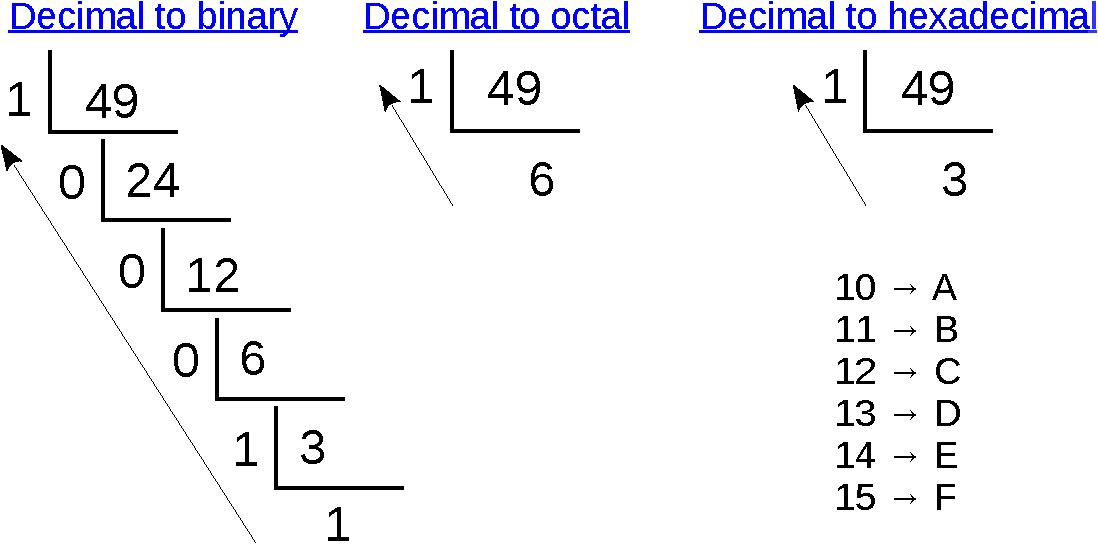
\includegraphics[width=0.85\linewidth]{figs/d2b.pdf}		
		\end{center}
	\end{figure}
\begin{itemize}
	\item {\textcolor{red}{Hints}: define a string char hmap[] =``0123456789ABCDEF''}
\end{itemize}
\end{frame}

\ifx\answer\defined
\begin{frame}[fragile]
\frametitle{Convert decimal to hexadecimal: the answer (1)}
\vspace{-0.3in}
\begin{columns}
\begin{column}{0.62\linewidth}
\begin{lstlisting}[xleftmargin=0.05\linewidth,linewidth=0.95\linewidth]
#include <stdio.h>
void dec2hexa(int n)
{
  int i = 0, d = n;
  int m = 0, t = 0;
  char hexa[64];
  char hmap[] = "0123456789ABCDEF";
  while(d > 0)
  {
      m = d%16;
      hexa[t] = hmap[m];
      d = d/16;
      t++;
  }
  printf("Hexa of %d is: 0x:", n);
  for(i = t-1; i>= 0; i--)
  {
      printf("%c", hexa[i]);
  }
  printf("\n");
}
\end{lstlisting}
\end{column}
\begin{column}{0.38\linewidth}
\begin{lstlisting}[firstnumber=14, linewidth=0.95\linewidth]
int main()
{
   int n=361005;
   dec2hexa(n);
   return 0;
}
\end{lstlisting}
\end{column}
\end{columns}
\end{frame}
\fi

\section{}
\end{document}
